\chapter{绪\hskip 0.4cm 论}
\label{chap1}
本章首先介绍了面向应急车辆优先通行的交通信号灯智能控制方法的研究背景及意义,接着阐述了国内相关科研状况,然后阐述了论文的研究内容及其学术贡献。最后提出了文章的组织架构。

%接着介绍了国内外相关研究现状,然后介绍了本文的研究内容以及学术贡献。最后给出了文章的组织结构。

\section{研究背景及意义}
在实际场景中,应急车辆是执行紧急任务的救护车、消防车或者警车等特种车辆,相比于其他车辆,它们具备更高的优先通行权以及具备更高的通行效率。根据国务院办公厅印发的文件,在充分保障交通安全的条件下,应急机动车不仅不受信号灯约束,而且不受行驶路线、方位、车速的约束,道路交通中其他机动车和行人必须给应急机动车让行\cite{chinaInfo}。 应急车辆优先通行是智慧交通的一个研究热点\cite{ITS_in_China, wulibin_vanet},其研究成果会推动缩短应急车辆的旅行时间,对挽救生命以及减少财产损失至关重要。随着物联网与智慧信息系统的发展,如今越来越多的人利用物联网技术,获取车辆信息以及交通灯信息\cite{chenhongyu,0TRAFFIC},通过V2V以及V2I技术实现车与车以及车与基础设施之间的通信\cite{nguyen2019combining, lijinyang, Oza_2020},也有人利用信息物理融合技术CPS(Cyber-Physical  Systems)提出交通灯信号控制的建议\cite{chang2020cps}。随着城市规模的增加,集中式交通方式也将遇到计算和通信上的困难,通过获取全局状态的集中式交通控制方法往往无法为应急车辆提供即时且可靠的信号控制策略,因此有人提出了分布式交通信号灯控制方案\cite{xuyang}。
%在实际场景中,应急车辆是执行紧急任务的救护车、消防车或者警车等特种车辆,相比于其他车辆,它们具备更高的优先通行权以及具备更高的通行效率。据国务院办公厅发布的通知,在能够保证安全的前提下,应急车辆不仅不受信号灯限制,也不受行驶路线、方向、速度的限制,道路中其他车辆和行人要为应急车辆让行\cite{chinaInfo}。 应急车辆优先通行是智慧交通的一个研究热点\cite{ITS_in_China, wulibin_vanet},其研究成果会推动缩短应急车辆的旅行时间,对挽救生命以及减少财产损失至关重要。随着物联网与智慧信息系统的发展,如今越来越多的人利用物联网技术,获取车辆信息以及交通灯信息\cite{chenhongyu,0TRAFFIC},通过V2V(Vehicle to Vehicle)以及V2I(Vehicle to Infrastructure)通信技术实现车与车以及车与基础设施之间的通信\cite{nguyen2019combining, lijinyang, Oza_2020},也有人利用信息物理融合技术CPS(Cyber-Physical  Systems)提出交通灯信号控制的建议\cite{chang2020cps}。随着城市交通规模的扩大,集中式交通控制方法将面临计算和通信上的难题,通过获取全局状态的集中式交通控制方法往往无法为应急车辆提供即时且可靠的信号控制策略,因此有人提出了分布式交通信号灯控制方案\cite{xuyang}。


%对于执行应急救援任务的应急车辆,在确保安全的前提下,不受行驶路线、行驶方向、行驶速度和信号灯的限制,其他车辆和行人应当让行\cite{chinaInfo}。 应急车辆优先通行是智慧交通的一个研究热点\cite{ITS_in_China, wulibin_vanet},其研究成果会推动缩短应急车辆的旅行时间,对挽救生命以及减少财产损失至关重要。随着物联网与智慧信息系统的发展,如今越来越多的人利用物联网技术,获取车辆信息以及交通灯信息\cite{chenhongyu,0TRAFFIC},通过V2V(Vehicle to Vehicle)以及V2I(Vehicle to Infrastructure)通信技术实现车与车以及车与基础设施之间的通信\cite{nguyen2019combining, lijinyang, Oza_2020},也有人利用信息物理融合技术CPS(Cyber-Physical Systems)提出交通灯信号控制的建议\cite{chang2020cps}。随着城市交通规模的扩大,传统的集中式交通控制方法会遇到计算和通信上的瓶颈,通过获取全局状态的集中式交通控制方法往往无法为应急车辆提供即时且可靠的信号控制策略,因此有人提出了分布式交通信号灯控制方案\cite{xuyang}。

图 \ref{fig:ambulance_road_live_map_1} 和图\ref{fig:ambulance_road_live_map_2}分别显示了普陀区中心医院附近和金沙江路救护车被前方其他车辆阻碍,无法继续向前行驶的道路实况。图\ref{fig:ambulance_road_live_map_1}由于道路狭窄,车辆密度大,导致道路拥挤,应急车辆只能缓慢向前行驶,这使得应急车辆到达目的地所需的旅行时间延长。图\ref{fig:ambulance_road_live_map_2}中其他车辆前方为十字交叉路口,且前方为红灯,因此救护车必须排队等候前方排队车辆清空后,才能通过交叉路口,该交叉口最高可导致救护车的旅行时间延长150秒,这严重威胁了病患人员的生命安全。

 \begin{figure}[ht]
	\centering
	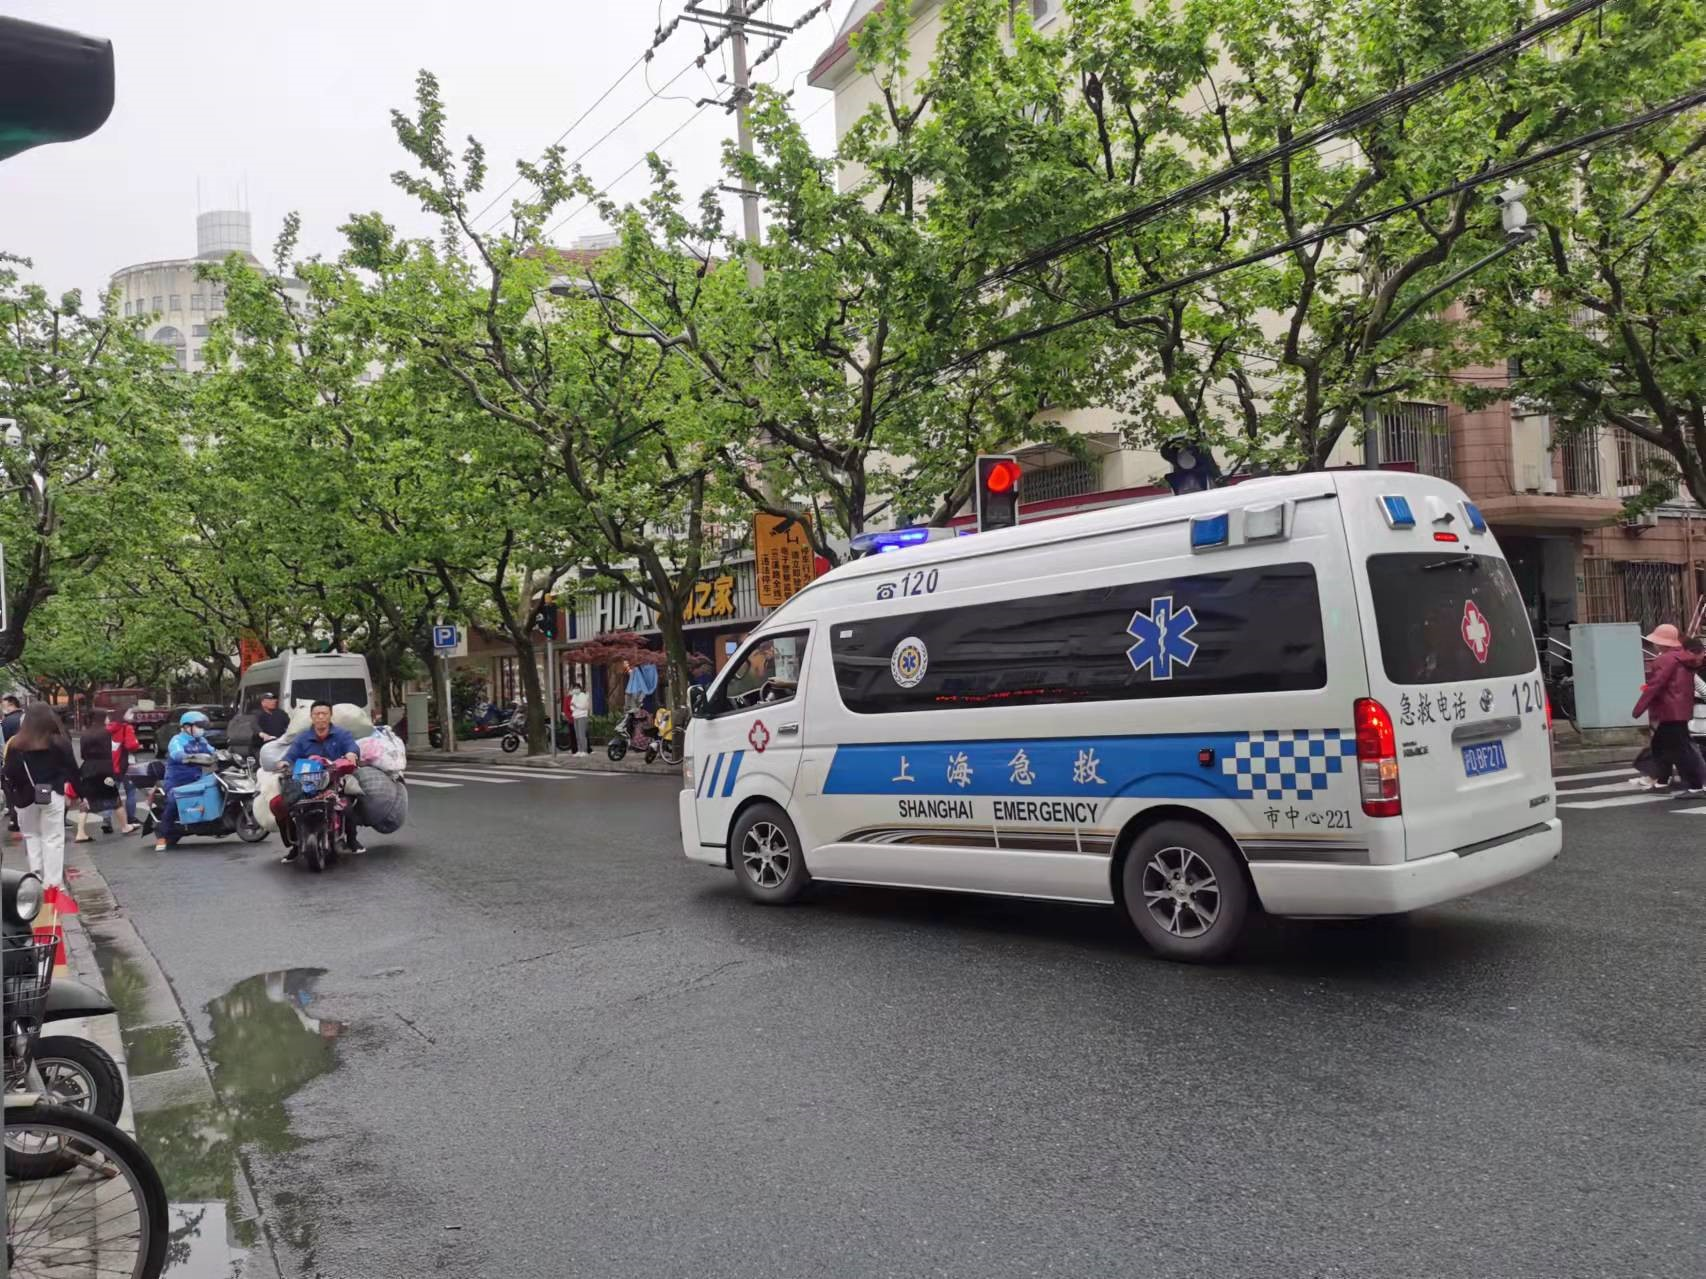
\includegraphics[width=\textwidth]{figures/ambulance_road_live_map_1.jpg}
	\caption{普陀区中心医院附近救护车救援道路实况图}
	\label{fig:ambulance_road_live_map_1}
\end{figure}

\begin{figure}[ht]
	\centering
	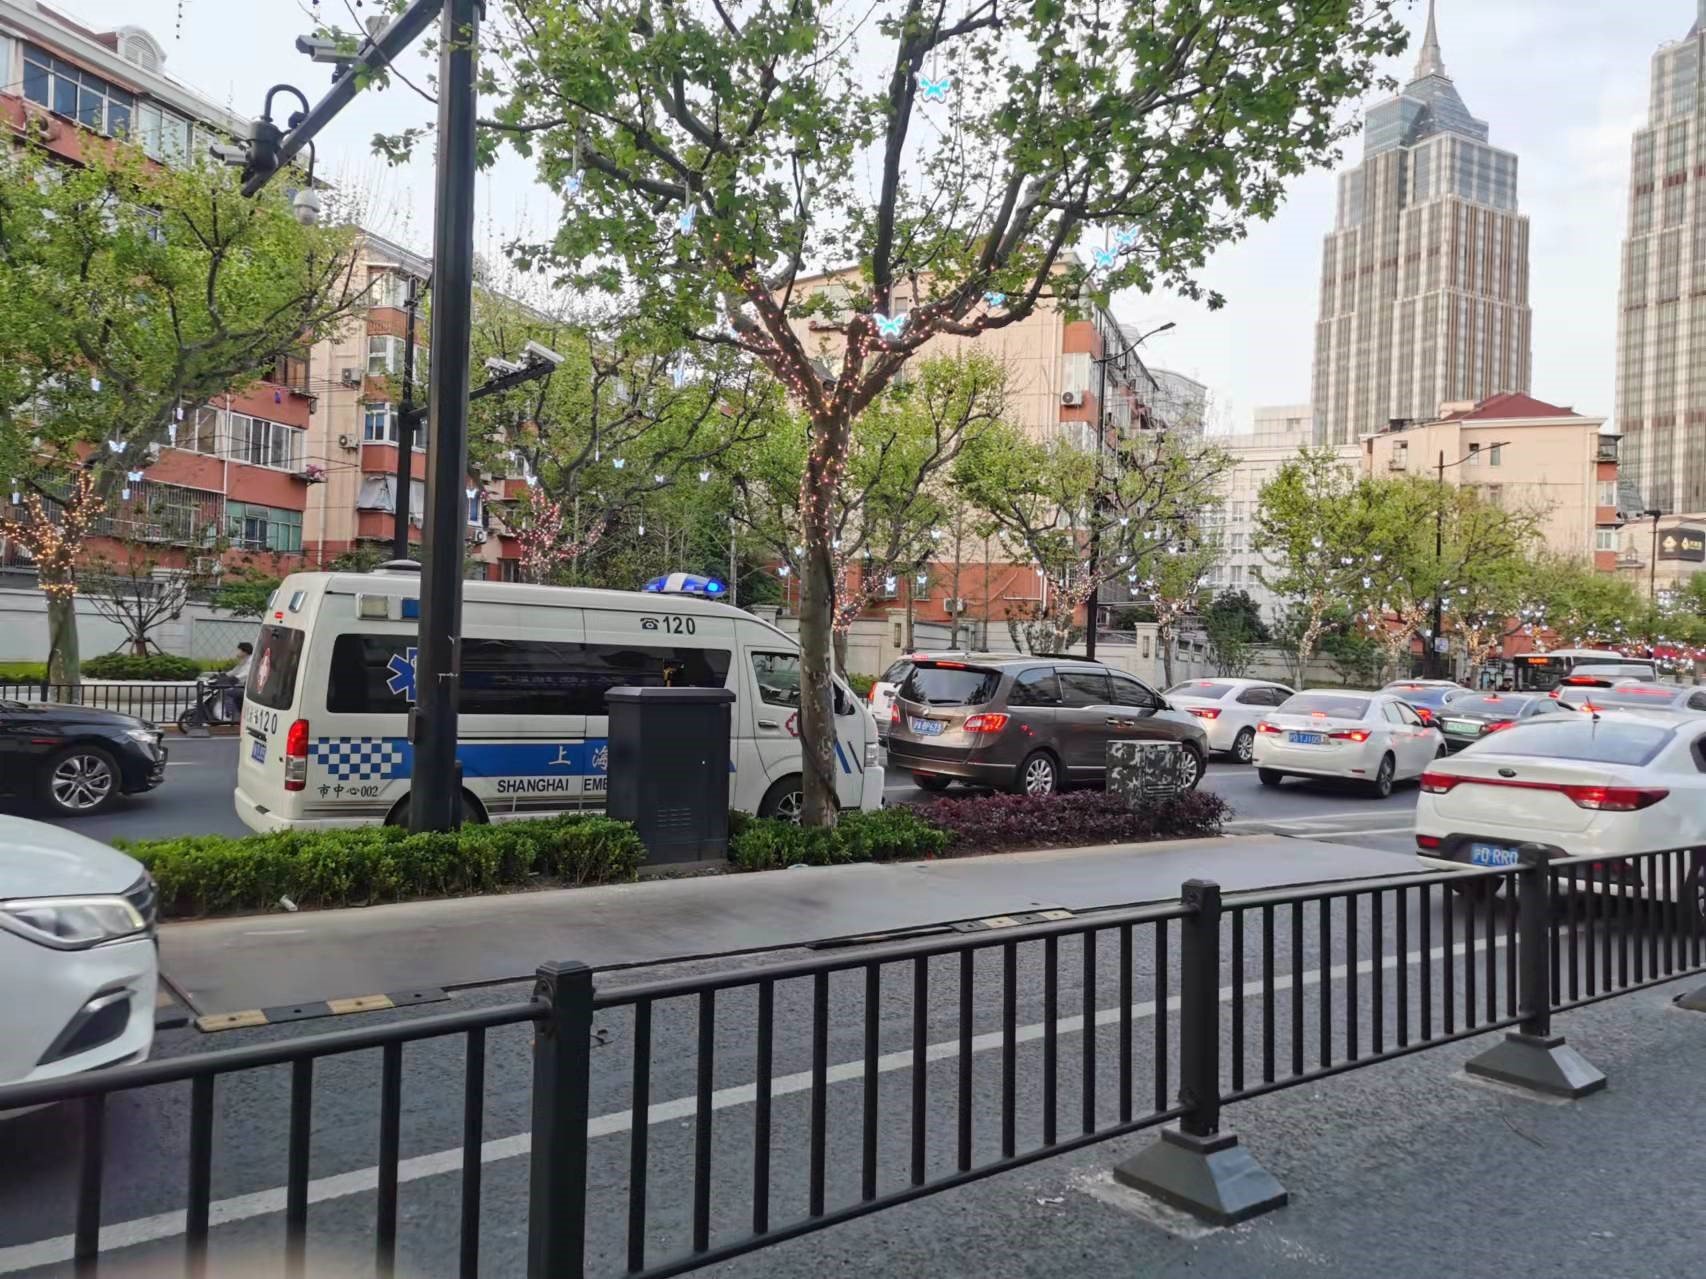
\includegraphics[width=\textwidth]{figures/ambulance_road_live_map_2.jpg}
	\caption{金沙江路附近救护车救援道路实况图}
	\label{fig:ambulance_road_live_map_2}
\end{figure}

%\section{研究意义}

随着城市交通规模的不断扩大,城市居民持有汽车总数不断飙升。据\cite{gongbao}显示,2020年年末,全中国拥有的公路营运汽车已经达到了1171.54万辆。人民日益增长的道路交通要求和不均衡不完善的路面设施之间的冲突造成了路面饱和度不断增加。道路饱和度上升不仅带来了日常交通拥堵,而且还会导致应急车辆在执行任务的过程中,其他车辆没有空间为应急车辆让行,阻碍应急车辆快速行驶,延长救援时间。应急车辆经过红绿灯路口时,大量且聚集的排队车辆会严重阻碍应急车辆的行进。提前清空红绿灯路口应急车辆之前的所有其他车辆,能够有效缩短应急车辆的旅行时间。有研究表明,在道路交通流量大的情况下,一个交叉口的信号抢占行为能够为应急车辆节省高达45s的时间\cite{wang_design_2013}。

%人民日益增长的交通需求与不平衡不充分的道路基础设施之间的矛盾导致了道路饱和度不断上升。

%缩短应急车辆的旅行时间对挽救生命和减少财产损失至关重要,在紧急情况下,几分钟的延迟就可能意味着生命的结束和巨额的财产损失。因此,全球各国政府都制定了应急救援时间目标,英国国家卫生服务系统NHS(National Health Service)为大多数的严重医疗呼救设定了8分钟的目标\cite{NHS};美国纽约规定紧急呼叫的应急救援时间为10分钟\cite{george_1};在新加坡有87.1\%的应急车辆能够在11分钟内到达目标位置\cite{Singapore}。随着中国城市化进程的加快,政府对缩短应急救援时间的需求也在不断上升。

缩短应急车辆的旅行时间对挽救生命和减少财产损失至关重要,在紧急情况下,几分钟的延迟就可能意味着生命的结束和巨额的财产损失。因此,全球各国政府都制定了应急救援时间目标,英国国家卫生服务系统(NHS)为大多数的严重医疗呼救设定了8分钟的目标\cite{NHS};美国纽约规定紧急呼叫的应急救援时间为10分钟\cite{george_1};在新加坡有87.1\%的应急车辆能够在11分钟内到达目标位置\cite{Singapore}。随着中国城市化进程的加快,政府对缩短应急救援时间的需求也在不断上升。


%虽然目前已有关于应急车辆信号抢占方面的研究,但传统的信号抢占法——当交通灯路口探测到应急车辆后,将应急车辆前进方向交通灯设置为绿灯的抢占方法,通常对道路中其他其他车辆影响较大\cite{2017Preemptive}。

%目前为止,尚未有研究既根据现实情况为应急车辆疏通道路,缩短应急车辆的旅行时间,又具备修复应急车辆的优先通行对整个交通流造成的影响的能力。因此,本文针对应急车辆的交通灯信号设计问题,研究如何合理地降低道路饱和度,从而在保证有效地缩短应急车辆旅行时间的前提下,尽可能减少应急车辆优先通行对整个交通流造成的影响。因此,研究针对应急车辆的交通灯信号设计问题,讨论如何合理地降低道路饱和度,如何有效地缩短应急车辆的旅行时间,以及降低应急车辆优先通行对整个交通造成的影响,具有十分重要的意义。

\section{国内外研究现状}
不同的国家以及研究人员都在不断尝试将新兴科技应用于智慧交通当中,这极大地促进了应急车辆优先通行的研究进程。美国\cite{2018Ghanim}、加拿大、澳大利亚、日本等国家都拥有自己的多车优先系统:日本的FAST系统为应急车辆提供最佳路径,并在交通灯路口为应急车辆提供优先通行权,当装有红外信标的应急车辆通过检测器时,交通灯就转为绿灯\cite{2019Constrained}。目前针对应急车辆优先通行的信号控制系统已经被广泛研究,并取得了不错的成果\cite{koike_study_2003}。与应急车辆优先通行的关键问题包括信号检测\cite{2016Chen,nellore2016traffic,2020Yao}、信号抢占以及应急车辆优先通行对整个交通流的影响。

随着物联网与智慧信息系统的发展,专用短程通信技术(DSRC)使得应急车辆能够与基础设施通信,从而提高了检测的准确性,与此同时,应急车辆配备GPS系统,能够发送实时位置信息。Ashish等人利用V2I动态暂停交通流的常规移动,为包含紧急车辆的进场提供绿灯,与此同时利用V2V通信使前面的车辆为紧急车辆让路\cite{Ashish_2021}。Ebizuka等人提出了评估应急车辆声源检测和识别的方法\cite{Ebizuka_2019}。Ismail等人利用arduino和蓝牙传感器,当紧急车辆接近红灯和排长队的红绿灯时,蓝牙传感器将向arduino发出信号以改变绿灯。目前将交叉口信号灯抽象为智能体已成为热门趋势,通过感知周围环境以控制交通灯信号周期\cite{2020Automated,2017Younes},如徐杨等人在\cite{xuyang}中给出了每一条交通灯路口采用一种非集中式的协同智能体来监控的信号控制方式。夏元清等人\cite{xiayuanqing}提出了一个智慧交通系统信息的物理融合云系统方案,包括了智慧交通系统的边缘控制技术。Shrivastava等人提供了一个开创性且实用的以服务器为中心的模型,使用全球定位系统 (GPS) 和调节交通信号的微控制器的基本手机应用程序实现抢占\cite{Shrivastava_2019}。Masoud等人提出了一种利用无电池无线传感器网络(WSN)来提高应急车辆的安全性和机动性的新方法\cite{Masoud_2017}。Peng等人提出了一种基于协同车辆基础设施系统(CVIS)的车队变道引导方法,使得其他车辆避开应急车辆\cite{Peng_2021}。



%不同的国家以及研究人员都在不断尝试将新兴科技应用于智慧交通当中,这极大地促进了应急车辆优先通行的研究进程。美国\cite{2018Ghanim}、加拿大、澳大利亚、日本等国家都拥有自己的多车优先系统:日本的FAST(Fast Emergency Vehicle Preemption)系统为应急车辆提供最佳路径,并在交通灯路口为应急车辆提供优先通行权,当装有红外信标的应急车辆通过检测器时,交通灯就转为绿灯\cite{2019Constrained}。随着物联网与智慧信息系统的发展,专用短程通信DSRC(Dedicated Short Range Communication)技术使得应急车辆能够与基础设施通信,从而提高了检测的准确性,与此同时,应急车辆配备GPS系统,能够发送实时位置信息。Ashish等人利用V2I动态暂停交通流的常规移动,为包含紧急车辆的进场提供绿灯,与此同时利用V2V通信使前面的车辆为紧急车辆让路\cite{Ashish_2021}。Ebizuka等人提出了评估应急车辆声源检测和识别的方法\cite{Ebizuka_2019}。Ismail等人利用arduino和蓝牙传感器,当紧急车辆接近红灯和排长队的红绿灯时,蓝牙传感器将向arduino发出信号以改变绿灯。目前将交叉口信号灯抽象为智能体已成为热门趋势,通过感知周围环境以控制交通灯信号周期\cite{2020Automated,2017Younes},如徐杨等人在\cite{xuyang}中给出了每一条交通灯路口采用一种非集中式的协同智能体来监控的信号控制方式。夏元清等人\cite{xiayuanqing}提出了一个智慧交通系统信息的物理融合云系统方案,包括了智慧交通系统的边缘控制技术。Shrivastava等人提供了一个开创性且实用的以服务器为中心的模型,使用全球定位系统 (GPS) 和调节交通信号的微控制器的基本手机应用程序实现抢占\cite{Shrivastava_2019}。Masoud等人提出了一种利用无电池无线传感器网络(WSN)来提高应急车辆的安全性和机动性的新方法\cite{Masoud_2017}。Peng等人提出了一种基于协同车辆基础设施系统(CVIS)的车队变道引导方法,使得其他车辆避开应急车辆\cite{Peng_2021}。

%如徐杨等人在[10]中给出了每一条交通灯路口采用一种非集中式的协同智能体来监控的信号控制方式。夏元清等人[26]提供了一个智慧交通系统信息的物理融合云系统方案,包括了智慧交通系统的边缘控制技术。

%\cite{Masoud_2017}紧急车辆优先 (EVP) 系统在重新确定信号交叉口的优先级方面发挥着关键作用。这个角色对于紧急车辆 (EV) 通过道路交叉口的安全和最小的旅行延误非常重要。不幸的是,目前在道路上使用的传统系统在成本、可靠性、可维护性和可扩展性方面存在缺陷。在本文中,提出了一种利用无电池无线传感器网络(WSN)来克服上述困难并提高应急车辆的安全性和机动性的新方法。基于收集树协议(CTP)设计了一种特殊用途的抢占协议作为数据收集服务。该协议称为 WSN-EVP,用于在跨交通路口的多跳树型拓扑中处理 EV 抢占请求。该模型根据预定义规则和优化参数运行,以应对高拓扑变化和快速响应时间要求。使用在 nesC 中编程的 TelosB 微尘的原型实现显示了在高干扰水平下具有高抢占精度的性能。

%\cite{Ismail_2019}在本文中,一种新的系统解决了紧急车辆通过红绿灯的问题,红绿灯堵塞了车辆排长队。一旦紧急车辆能够轻松通过红绿灯,这将节省紧急车辆的行驶,并根据紧急车辆的类型(即火灾或生命)挽救情况。这个新系统利用了arduino和蓝牙传感器的优势。客户端蓝牙连接到紧急车辆,主蓝牙和 arduino 位于红绿灯处。在这个系统中,当紧急车辆接近红灯和排长队的红绿灯时,蓝牙传感器将向arduino发出信号以改变绿灯。

%目前的信号抢占策略丰富多样,主要分为侵入式信号抢占和非侵入式信号抢占两类。前者通过检测应急车辆,当应急车辆到达交通灯路口时,将交通灯设置为绿灯。后者通过改变相位周期,使得应急车辆到达交通灯路口时刚好遇到绿灯。

%Hashim等人\cite{hashim}提出了一种能够对应急车辆发出的无线信号做出快速反应的交通信号控制系统。
%\subsection{信号抢占相关研究}
目前的信号抢占策略丰富多样。Qin等人\cite{qin_control_2012}提出了一种信号控制策略,当传感器检测到应急车辆时,自动将交通灯设置为紧急抢占EVSP(emergency vehicle signal pre-emption)模式,在应急车辆通过交通灯路口后,恢复到正常模式。Noori 等人\cite{noori2016connected}提出了一种基于连接车辆的控制策略,在为应急车辆提供绿灯的同时能够清空应急车辆前方的排队车辆。闵万里等人\cite{min}提出了弹性信号抢占,通过重新规划相位周期时间使得应急车辆到达交叉口时刚好遇到绿灯。Kang等人\cite{wenwen_kang_traffic_2014}提出了紧急车辆信号协调方法EVSC(Emergency Vehicle Signal Coordination),通过修改相位偏移为应急车辆提供“绿波”效应,保证应急车辆在一片区域内一路绿灯通行。Petrica等人提出了基于车辆类型、路口等待队列长度和多路口通信的优先分配红绿灯算法\cite{Petrica_2021}。Obrusnik等人提出了应用于十字路口的信号抢占方法,能够使得抢占时间尽可能短\cite{Obrusnik_2020}。Shaaban等人还提供了一个用于最优路线选取和应急车辆抢占的联合策略,所建议的方法在所有应急车离开其原点之前为其选定最佳路线,然后在适当的时机激活对每个路口的抢占,使其在应急车辆到达之前清除路口\cite{Shaaban_2019}。Cao等人提出了一种以应急车辆为中心的交通信号控制,它关注应急车辆的性能,同时最大限度地减少冲突方向对交通的负面影响\cite{Cao_2019}。Mu等人设计了一个由监控子系统、相位时间确定子系统和相位切换控制子系统组成的应急车辆抢占优化控制系统\cite{Mu_2018}。

%Mu等人还产品设计了一套由监测子系统、相位时刻确认子系统和相位切换监测子系统所构成的应急车辆抢占优化管理系统[38]。

%\cite{Peng_2021}为保证应急车辆能够更安全、高效地到达事故现场,本文提出了一种基于协同车辆基础设施系统(CVIS)的车队变道引导方法,以避开应急车辆。提出了三种协同变道策略来保证从后方接近的应急车辆快速通过目标车道内对应的三种场景:无车辆、车辆稀少和车辆排。协同变道策略引导应急车辆前方的车辆排和其他车辆目标车道改变它们的速度,调整车辆之间的距离,并根据轨迹规划完成车道变换。


%\cite{Mu_2018}本文重点关注使用定时彩色 Petri 网 (TCPN) 研究应急车辆 (EV) 抢占控制问题。采用TCPN建立由三个子模型组成的城市交通网络模型,即交通流模型、交通信号显示与相位切换模型、交通信号切换控制模型。设计了一个由监控子系统、相位时间确定子系统和相位切换控制子系统组成的电动汽车抢占优化控制系统。提出了电动汽车在路段上行驶速度的计算方法,给出了确定当前阶段和其他阶段实际绿灯时间的方法。进行了一些计算比较来验证信号抢占控制策略,


%\cite{Obrusnik_2020}记录了一种在交通信号灯控制的十字路口抢占紧急车辆的新方法。该方法依赖于应急车辆和交通信号灯控制器之间的无线车辆到基础设施 (V2I) 通信、对队列中车辆数量的准确估计的可用性以及队列排放动力学的数学模型。与一些偶尔部署的方法在紧急车辆出现在距交叉口预定距离的瞬间触发抢占不同,所提出的方法使激活时刻适应实际交通状况,使抢占时间尽可能短,从而减少影响在其他交通。

%\cite{Shaaban_2019}紧急车辆抢占 (EVP) 旨在通过在途中创建绿波,为通过信号交叉口网络前往事发地点的紧急车辆 (EV) 提供通行权。EVP 系统的设计目标有两个:第一,避免阻碍 EV 在道路和交叉路口的通行;第二,减少抢占对一般交通的负面影响。通过选择合适的抢占策略,可以将 EVP 对正常流量的负面影响降到最低。早先提出的EVP方案旨在最大限度地减少EV的行驶时间,而没有或很少考虑EVP对正常交通的负面影响。在这项研究中,开发了一种用于最优路径选择和 EV 抢占的联合策略。所提出的方案在 EV 离开其原点之前为其选择最佳路径,然后在正确的时间激活每个路口的抢占,以在 EV 到达之前清除路口。提议的EVP 方案还旨在最小化EVP 在两个阶段(即路径选择阶段和抢占阶段)对正常流量的影响。该方法的一个主要优点是,一旦选择了最佳路径,紧急信息可以通过EV路径中的车对车和车对基础设施通信传播给其他车辆,以清除整个路径或接近车道。该策略使用微观模拟环境进行了测试,用于真实的交通网络。研究结果表明,电动汽车的行驶时间大大减少,同时将抢占对正常交通的影响降至最低。提议的策略和评估程序有助于相应的机构和从业者评估实施抢占对现有或提议的干线的影响。

%\cite{Cao_2019}提出了一种以应急车辆为中心的交通信号控制,它关注应急车辆的性能,同时最大限度地减少冲突方向对交通的负面影响。 

%\subsection{应急车辆优先通行交通影响相关研究}

为了降低应急车辆优先通行对整个交通流造成的影响,很多研究者通过改进信号抢占方法,减少对其他车辆的影响。如Wang等人\cite{wang_design_2013}提出了多层模糊模型,综合考虑应急车辆抢占需求强度以及应急车辆优先对其他车辆的影响程度。邵明莉等人\cite{shaomingli}通过深度强化学习方法,对应急车辆与其他车辆赋予不同的优先级,提出了针对应急车辆的降低道路饱和度的算法,缩短了应急车辆的旅行时间。Qin等人\cite{qin_control_2012}设计的信号恢复策略在应急车辆通过交通灯路口后恢复交通流能够一定程度上弥补应急车辆优先对整个交通造成的影响。闫飞等人\cite{yanfei}为使得交叉口各方向趋于均衡,使用了迭代学习控制方法。Hajiebrahimi等人提出了一种基于模糊规则的交通信号计时系统(STC),用于解决应急车辆的行程延误问题。Paruchuri等人提出了一种自适应交通抢占系统(APT),利用对交通网络中当前交通状况的了解,自适应地抢占应急车辆路径上信号灯,以最小化应急车辆的停车延误,同时最大限度地减少系统中非应急车辆的延误。

%\cite{Oza_2020}有效的交通控制仍然是一项具有挑战性的任务,尤其是在特殊事件期间和之后,例如紧急车辆穿越或因车辆故障而阻塞的链接。虽然现有方法旨在减少旅行延误,但它们并未考虑从交通网络中断造成的溢出中恢复。本文 (1) 提出了一种优化算法,在确保正常运营期间不会发生溢出的同时,最大化通过道路网络的交通流量,(2) 提出了一种有效的、可预测的缓解策略,以从特殊事件引起的溢出中恢复,并且可能已经通过网络中的多个链接和/或交叉点传播,并且 (3) 提供了与所提出的技术相关的最坏情况等待时间界限以及恢复时间界限。与现有方法相比,我们的最优策略显示最坏情况下的旅行时间缩短了 53.2%。此外,我们的缓解策略可以从通过网络中多个链路传播的溢出中恢复,比现有方法快 50.9%。
%In this paper, we document a novel method for emergency vehicle preemption at an intersection controlled by traffic lights. The method relies on wireless vehicle-to-infrastructure (V2I) communication between the emergency vehicle and the traffic lights controller, availability of an accurate estimate of the number of vehicles in the queue, and a mathematical model of dynamics of discharging of the queue. Unlike some occasionally deployed methods that trigger the preemption the instant that the emergency vehicle appears at a prespecified distance from the intersection, the proposed method adapts the activation moment to the actual traffic conditions so that the preemption is as short as possible, thus reducing the impact on the other traffic. The method has been finetuned using numerical simulations in SUMO simulator and experimentally verified in real urban traffic. Copyright (C) 2020 The Authors.






%\cite{Hajiebrahimi_2018} 本文提出了一种基于模糊规则的交通信号计时系统,称为 STC,用于解决紧急车辆的行程延误问题。该方法将专家的知识制定为规则,并利用模糊集将语言参数(例如估计到达时间和当前交通量)作为输入。结果是信号定时过程减少了紧急车辆路线沿线的交通负荷。

%\cite{Paruchuri_2017}提出了一种用于智能交通系统中紧急车辆的自适应交通抢占(APT)系统。我们利用对交通系统中当前交通状况的了解,自适应地抢占电动汽车路径上的信号灯处的交通,以最小化,如果不能消除电动汽车的停车延误,同时最大限度地减少系统中非紧急车辆的延误。

%\section{存在的问题}
%虽然面向应急车辆优先通行的交通灯控制策略已经被广泛研究,但是很少有人考虑到在道路比较拥挤的情况下,应急车辆前方的其他车辆阻碍了应急车辆的行进,需要提前为应急车辆降低道路饱和度,以提供应急车辆快速行驶的条件。侵入式信号抢占对其他车辆的影响较大,而非侵入式抢占受到绿灯时长以及车速动态变动的限制,抢占成功率不如侵入式抢占。同时目前很少有研究考虑到,如何修复应急车辆优先通行对整个交通造成的影响\cite{Shaaban_2019}。此外,目前的研究大多仅关注应急车辆前方的单个交叉口内的排队车辆,而不考虑应急车辆即将通行的其他交叉口,这种策略可能导致排队车辆来不及清空,应急车辆就已经到达交叉路口。因此预测排队车辆\cite{fengning},以及关注应急车辆即将通行的多个交叉口同样至关重要。
\section{本文工作及主要贡献}
为了缩短应急救援时间,并减少应急车辆优先对整个交通流造成的影响。本文提出了一种面向应急车辆优先通行的“绿波带”信号控制方法,本方法包含提前降低道路饱和度、为应急车辆提供信号抢占以及恢复整个交通流三个阶段保障应急车辆一路快速绿灯通行。
\begin{enumerate}
	\item 提前降低道路饱和度:根据应急响应等级、路段拥堵等级以及时间紧迫等级得出降低道路饱和度的迫切程度值,再根据降低道路饱和度迫切程度值合理地延长目标相位绿灯时间;
	
	%,在交叉灯路口,一个信号相位是指交叉路口各入口车道不同方向所显示的红黄绿三种灯色组合,目标相位(Target Phase,简称TP)为应急车辆入口车道方向显示绿灯的信号相位,在该信号相位下,应急车辆能够直接通过路口而无需停车;
	\item 信号抢占:为应急车辆提供了非侵入式抢占与侵入式抢占相结合的信号控制方法,一种是基于二次规划的非侵入式信号抢占方法,通过改变信号周期与相位时间使得应急车辆到达交通灯路口时刚好遇到绿灯,即应急车辆到达路口时,交通灯刚好处于目标相位,当第一种方法无法得出最优解时,本文中第二种信号抢占方法侵入式信号抢占方法将作为补充,以确保应急车辆到达交通灯路口时前方无排队车辆,且交通灯处于目标相位;
	\item 恢复交通流:通过线性规划方法,重新规划信号周期与交通灯路口各相位绿灯时间,在最短的时间内使得路口各方向排队车辆数小于等于没有应急车辆优先通行情况下的平均排队车辆数。
\end{enumerate}

为了验证本文方法的有效性,我们在城市交通模拟器SUMO\cite{behrisch2011sumo}中对路网中的多个十字路口与T型路口进行实验,结果表明本方法能够有效降低应急车辆的通行时间,并有效缓解应急车辆优先对整个交通流造成的干扰。

%第一阶段降低道路饱和度;为确保应急车辆到达交通灯路口时能快速通过交叉口,第二阶段第三阶段此外,在本文中,每个路口交通灯由一个智能体控制,智能体与应急车辆进行沟通。为了验证本文方法的有效性,我们在城市交通模拟器SUMO\cite{2011SUMO}中对路网中的多个十字路口与T型路口进行实验,结果表明本方法能够有效降低应急车辆的旅行时间,并有效缓解应急车辆优先对整个交通流造成的影响。

\section{文章组织框架}
第一章绪论,介绍了研究背景及意义、国内外研究现状以及本文工作及主要贡献。
%第一章绪论,介绍了研究的背景及意义,介绍了面向应急车辆的信号控制方法的国内外研究现状,并提出了本文的工作及主要贡献。

%第二章介绍了本文研究中涉及的相关知识,包括饱和流量、饱和流率、信号相位和绿波带等交通工程相关知识,以及K-Means均值聚类算法、线性规划和二次规划等机器学习相关知识。
第二章预备知识,介绍了饱和流量、饱和流率、信号相位和“绿波带”等交通工程相关知识,以及K-Means均值聚类算法和二次规划算法。

第三章面向应急车辆的“绿波带”模型,介绍了本文方法的整体框架及工作流程,包括了路网建模、信号控制各阶段的工作契机,以及降低道路饱和度、信号抢占以及恢复交通流各阶段的的转换。

第四章交通信号灯控制方法,介绍了降低道路饱和度、信号抢占以及恢复交通流各阶段的工作原理及算法。首先提出了根据应急响应等级、路段拥堵等级以及时间紧迫等级确定降低道路饱和度等级以确保非应急车辆能够为应急车辆让行。然后提出了非侵入式抢占与侵入式抢占相结合的信号抢占方法,保证应急车辆直接通过交叉口无需停车。最后通过线性规划方法将交叉口各方向交通流恢复到信号抢占之前的状态。

第五章基于SUMO平台的实验评估与分析,对本文方法进行了实验评估与分析,在城市交通模拟平台SUMO中对本文方法与已有的方法进行对比,验证了本方法能够为应急车辆提供一路绿灯的快速通行方案,缩短了应急车辆的旅行时间,并能够实现应急车辆优先对整个交通流的影响得到修复。

%第五章基于SUMO平台的实验评估与分析,对本文方法进行了实验评估与分析,在城市交通模拟平台SUMO\cite{2011SUMO}中对本文方法与已有的方法进行对比,验证了本方法能够为应急车辆提供一路绿灯的快速通行方案,缩短了应急车辆的旅行时间,并能够实现应急车辆优先对整个交通流的影响得到修复。

第六章总结和展望,对本文工作做出总结并给出了未来的工作展望。


%论文其他部分内容组织如下:第1节主要介绍了与本文相关的交通灯信号控制方法;第2节阐述了本文提出的面向应急车辆优先通行的交通灯信号控制方法,阐述了信号灯在降低道路饱和度、为应急车辆提供信号抢占以及恢复整个交通流三个阶段中的详细设计方法;第3节详细描述了本文交通灯信号控制方法中的第一阶段,即降低道路饱和度阶段;第4节详细描述了本文交通信号控制方法中的第二阶段,即为应急车辆提供信号抢占阶段;第5节详细解释了本文交通信号控制方法中的第三阶段,即恢复整个交通流;第6节通过在城市交通模拟器SUMO平台中进行对比实验,第7节对本文工作做出总结并给出了未来的工作展望。




